% Drawing 67/01-3 -- folder 67, batch 01, archive page 3 (PDF page 4).
% Transcription: à gauche, trois croquis de cylindres traversés de cercles et de courbes, le troisième biffé
% Kind: cylinders crossed by circles and curves. Method 2 (schematic redraw from the facsimile). Status: ok.
% Notes: Two pencil cylinders, each between two horizontal lines and crossed by three closed curves. Omitted as struck: the third cylinder (bottom left), struck through by oblique strokes. The marginal words on the right ("cylindre ...") are left out. Issue 128, 2026-11-09: struck material left out after a fresh check of the facsimile (struck-out material is not drawn). Redrawn 2026-11-09 (issue 128): to check again.
% Coordinates: 1 unit = 1 mm = 1/100 of the crop width (bbox in page fractions: [0.15, 0.62, 0.72, 0.8]).
% Redrawn by Claude (claude-opus-5-5), issue #73, 2026-11-07; not checked by a human; not compiled (no TeX in the session).
% Rights: reproduces part of the work -- behind RENDER_TRANSCRIPTS, never published by itself.
\documentclass[tikz,border=3pt]{standalone}
\usepackage{amsmath,amssymb}
\usetikzlibrary{patterns,arrows.meta}
\tikzset{pencil/.style={black!45}, struck/.style={black!35}, mark/.style={circle,draw,inner sep=1.3pt}, pt/.style={circle,fill,inner sep=0.9pt}, opt/.style={circle,draw,fill=white,inner sep=1.1pt}}
\begin{document}
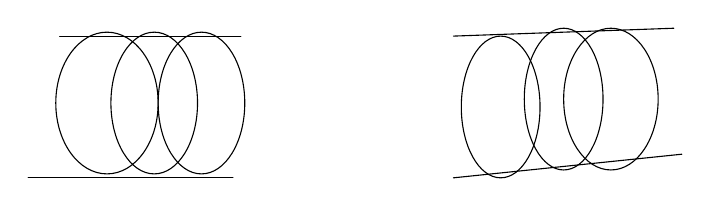
\begin{tikzpicture}[x=1mm,y=1mm,line cap=round,line join=round,font=\scriptsize]
\draw (14,-7) -- (37,-7);
\draw (10,-25) -- (36,-25);
\draw (20,-15.5) ellipse[x radius=6.5, y radius=9];
\draw (26,-15.5) ellipse[x radius=5.5, y radius=9];
\draw (32,-15.5) ellipse[x radius=5.5, y radius=9];
\draw (64,-7) -- (92,-6);
\draw (64,-25) -- (93,-22);
\draw (70,-16) ellipse[x radius=5, y radius=9];
\draw (78,-15) ellipse[x radius=5, y radius=9];
\draw (84,-15) ellipse[x radius=6, y radius=9];
\end{tikzpicture}
\end{document}
